% Template - https://sanskrit.uohyd.ac.in/18WSC/Style_files/CS_and_DH.tex
\providecommand{\tightlist}{%
  \setlength{\itemsep}{0pt}\setlength{\parskip}{0pt}}

\documentclass[11pt]{article}
\usepackage{scl}
\usepackage{times}
\usepackage{url}
\usepackage{latexsym}
\usepackage{lineno}

\usepackage{fontspec, xunicode, xltxtra}
\newfontfamily\skt[Script=Devanagari]{Sanskrit 2003}
\setmonofont{Sanskrit 2003}


\title{A general Dictionary distribution framework}

\author{
  Vishvas Vasuki \\
  Dyugaṅgā, Beṅgaḷūru \\
  {\tt https://sanskrit.github.io/groups/dyuganga/}
\\}

\date{}

\begin{document}
\maketitle
%\linenumbers
\begin{abstract}
Dictionaries are the constant companions of scholars and students, and there are lot of them (some being continuously updated). They are often consumed offline, on a variety of devices including one's phone. We describe a general dictionary distribution framework which serves hundreds of such dictionaries to a sizable user community.
\end{abstract}

\section{Motivation}
Today's scholars and students frequently want to refer dictionaries on electronic devices ranging from desktop computers to phones and voice-AI devices like Alexa. Dictionaries of interest may be large in number and size. For example, there are hundreds of dictionaries of interest to Indological scholars accross a variety of languages and topics. Furthermore, some of these dictionaries are constantly being updated. Beyond that, a good subset of subset of such users want such dictionaries to be available offline.

This being the case, it becomes problematic to curate, distribute and update such dictionaries for the convenience of both creators and users. We present an open source and extensible system to address this problem. Some of its features are listed below.

\begin{itemize}
\tightlist
\item \textbf{For creators}
\begin{itemize}
\tightlist
\item Easy to publish a new dictionary or update an old one.
\item Support for some basic HTML formatting.
\item Ability to link to references and solicit feedback/ corrections.
\end{itemize}

\item \textbf{For readers}
\begin{itemize}
\tightlist
\item Easy to install dictionaries.
\item Easy to selectively update only obsolete dictionaries (saving download cost and effort).
\item Easy to only select dictionaries from particular categories.
\item Available across devices, and easily extensible.
\end{itemize}
\end{itemize}

This system is currently used to publish hundreds of dictionaries across over a dozen languages (Listable via \cite{stardict_index}), and is patronized by a sizeable user community.

\begin{figure}[h]
\caption{Screenshot from GoldenDict}
\centering
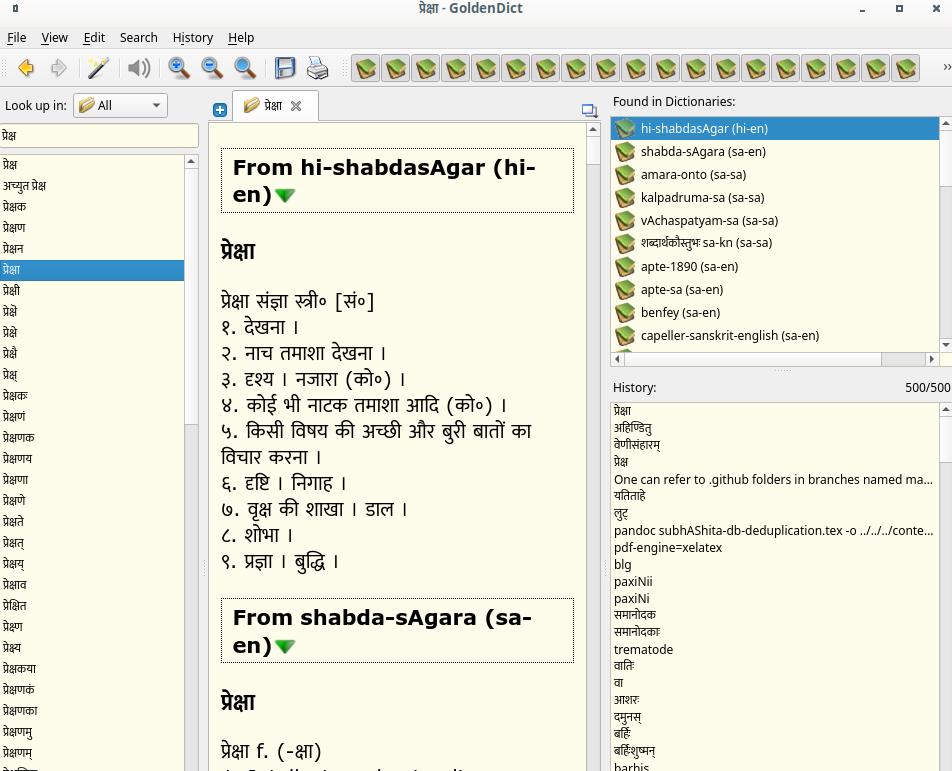
\includegraphics[width=1.0\textwidth]{images/goldendict-desktop-screenshot}
\end{figure}


\section{Future work}

\bibliographystyle{acl}
\bibliography{dict-distribution}
\end{document}